\section{Passeggiata Aleatoria}

Data un'equazione della forma
\begin{equation}\label{eq:ricorsiva}
  a x_{n+1} + b x_{n} + c x_{n-1} = 0 
\end{equation}
questa è detta \textbf{ricorsiva} e per risolverla si usano tecniche diverse.

Un esempio tale è la successione di Fibonacci:
\[
  \begin{cases}{}
      x_{n+1} = x_{n} + x_{n-1} \\
      x_{0} = 0 \\
      x_{1} = 1
  \end{cases}
\]
Per risolvere~\eqref{eq:ricorsiva} si può (ad esempio) supponere che la soluzione sia della forma
\(x_{n} = \lambda^{n}\). Allora sostituendo otteniamo
\[
  \lambda^{n-1} {\left( a \lambda^{2} + b \lambda + c \right)} = 0
\]
Allora otteniamo che, date \(\lambda_{1}\) e \(\lambda_{2}\) le radici del
polinomio di secondo grado, due possibili soluzioni sono \(x_{n} =
\lambda_{1}^{n}\) e \(x_{n} = \lambda_{2}^{n}\). Dato ora che lo spazio delle
soluzioni è lineare, ogni soluzione è della forma \(x_{n} = A \lambda_{1}^{n} +
B \lambda_{2}^{n}\). Infine, per determinare le costanti si possono utilizzare i
dati iniziali. Ovviamente se \(\lambda_{1} = \lambda_{2}\) dobbiamo fare qualche
passaggio in più per ottenere due soluzioni indipendenti, similmente a come
risolvevamo le equazioni differenziali.

\subsection{Rovina del Giocatore}

nel caso \(p\neq \frac{1}{2}\), l'equazione di interesse è 
\[
  u{(i)} = p\, u {(i+1 )} + {(1-p)} \,u {(i-1)} \quad\quad\quad 1 \le  i \le N = \alpha +
  \beta
\]
Questo è un esempio di equazione di tipo ricorsivo. Possiamo dunque applicare un
metodo simile a quello visto per la versione generale~\eqref{eq:ricorsiva} e
consideriamo i dati iniziali. \(u{(0)}\) è la probabilità di rovinarsi partendo
al tempo 0, che dunque è 1. E la probabilità di rovinarsi a \(n\), quando vengo
assorbito, è 0. Allora si tratta di risolvere
\[
  \begin{cases}{}
      u{(i)} = p\, u{(i+1 )} + {(1-p)}\, u{(i-1)}\\
      u{(0)} = 1 \quad ; \quad u{(n)} = 0
  \end{cases}
\]
per trovare una soluzione dunque facciamo come prima, dunque poniamo \(u{(i)} =
y^{i}\), trovando dunque \(p y^2 - y + 1-p = 0\). Questa ha due radici
\[
  y_{1} = 1 \quad y_{2} = \frac{1-p}{p}
\]
se \(y_{1} \neq y_{2}\), dunque \(p \neq \frac{1}{2}\), allora possiamo scrivere
che la soluzione generica è 
\[
  u{(i)} = A + B {\left( \frac{1-p}{p} \right)} ^{i} 
\]
con \(A\) e \(B\) costanti. Dalle condizioni al bordo troviamo che
\[
    \begin{cases}{}
        u{(0)} = 1\\
        u{(N)} = 0
    \end{cases}
    \implies 
    \begin{cases}{}
        A+B = 1\\
        0 = A + B {\left( \frac{1-p}{p} \right)} ^{N}
    \end{cases}
    \implies 
    \begin{cases}{}
        A = 
    \end{cases}
\]
e la soluzione è dunque data da 
\[
  u{(i)} = \frac{{\left( \frac{1-p}{p} \right)} ^{N} - {\left( \frac{1-p}{p}
  \right)} ^{i}}{{\left( \frac{1-p}{p} \right)} ^{N} - 1}
\]

\subsection{Durata del gioco}
Una possibile domanda è: \emph{Mediamente quanto dura il gioco?}

Per possibile a questa domanda devo introdurre le V.A. che descrivono i tempi di
raggiungimento di \(0\) o \(N\). Chiamando questi \(T_{0}\) e \(T_N\) definisco
\(T = \inf \{T_{0}, T_{n}\} \) sono dunque interessato a \(\mathbb{E}{(T \;|\;
X_{0} = i)} = \mathbb{E}_i{(T)}\). Un'idea è trovare un'equazione ricorsiva per
\(\mathbb{E}_i{(T)}\) 
\begin{center}
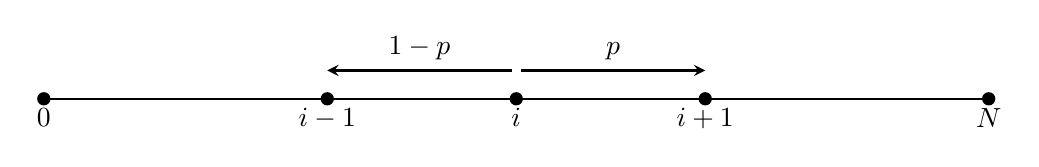
\begin{tikzpicture}[>=stealth, scale=1.2]

    % Draw the line
    \draw[thick] (0,0) -- (10,0);

    % Points
    \fill (0,0) circle (2pt) node[below] {$0$};
    \fill (3,0) circle (2pt) node[below] {$i-1$};
    \fill (5,0) circle (2pt) node[below] {$i$};
    \fill (7,0) circle (2pt) node[below] {$i+1$};
    \fill (10,0) circle (2pt) node[below] {$N$};

    % Arrows for probabilities
    \draw[->, thick] (5.05,0.3) -- (7,0.3) node[midway, above] {$p$};
    \draw[->, thick] (4.95,0.3) -- (3,0.3) node[midway, above] {$1-p$};

\end{tikzpicture}
\end{center}

L'equazione per il tempo è simile a quella di prima, con aggiunto un istante
ogni volta:
\[
  \mathbb{E}_i{(T)} = 1 + p\, \mathbb{E}_{i+1} {(T)} + {(1-p)} \mathbb{E}_{i-1}
  {(T)}
\]
con dati al bordo stavolta che sono \(\mathbb{E}_0 {(T)} = \mathbb{E}_N{(T)} =
0\). Senza stare a vedere i conti, nel caso simmetrico \(p = \frac{1}{2}\) vale
allora che
\[
  \mathbb{E}_i{(T)} = i {(N-i)}
\]
Dunque se parto che ricchezza \(\alpha\) e \(N = \alpha + \beta\), allora ho
\(\mathbb{E}_i {(T)} = \alpha \beta\) 

\begin{remark}{}
    Se \(\beta \gg \alpha\) ad esempio umano vs casinò, allora la probabilità
    che io mi rovini è \(u{(\alpha)} \approx 1\) ma \(\mathbb{E}_{\alpha} {(T)}
    \approx \alpha\beta\) che possibilmente è molto alto.
\end{remark}

